%!TEX root = ../trabajo.tex
\capitulo{Marco Metodológico}
A continuación se explicarán los aspectos metodológicos que se emplearán para la consecución de los objetivos específicos planteados. 

\seccion{Tipo de Investigación}
\citet{simon1996sciences}, consideró el diseño como un proceso científico, dada la necesidad existente de un método general que sea utilizado para diseñar o proyectar; a esta ciencia del diseño, la denominó ciencia de lo artificial, que es distinta del campo de las Ciencias de la Naturaleza y diferente también del ámbito de las Ciencias Sociales \cite[pp. 42-43]{gonzalez2007configuracion}. \citet[pp. 567-569]{hurtado2012metodologia}, afirma que en algunos contextos, a la investigación proyectiva también se le llama investigación tecnológica, estas  investigaciones conducen a inventos, programas, diseños o creaciones dirigidas a cubrir una determinada necesidad.
\\
\\ 
Desde otro ángulo, \citet{cordoba2005investigacion} afirma que las perspectivas metodológicas de la investigación en lo social ocurren de dos (2) maneras, estas son la cuantitativa y la cualitativa, pero si se parte de que existe la necesidad de transformar, entonces ni lo cuantitativo ni lo cualitativo son suficientes, de allí que se recurra a lo tecnológico. Definiendo a la investigación tecnológica como aquella que tiene por fin obtener un conocimiento para lograr modificar la realidad en estudio, vinculando la investigación y la transformación. La investigación tecnológica, denominada también como investigar, idear e innovar, persigue un conocimiento práctico, que sea más un conjunto de instrucciones a seguir para transformar el objeto, que explicaciones teóricas respecto a las cualidades del mismo. \\
\\
Esta investigación se desarrollará desde la perspectiva de la investigación tecnológica con un enfoque en ciencia del diseño, bajo la modalidad de investigación de Estudios de Proyectos, según el Manual para la Elaboración del Trabajo Conducente a Grado Académico de Especialización, Maestría y Doctorado,\citet[p. 63]{UCLAmanual2002}, donde se define de la siguiente manera:
\begin{citatextual}
`` Se entenderá por estudios de proyectos una proposición sustentada en un modelo viable para resolver un problema práctico planteado, tendente a satisfacer necesidades institucionales o sociales y pueden referirse a la formulación de políticas, programas, tecnología, métodos y procesos''.
\end{citatextual}
\\
Adicionalmente se destaca que el presente estudio se fundamentará en investigación monográfica documental.

\seccion{Diseño de la Investigación}

El término diseño de investigación se refiere al plan o estrategia que se desarrolla para obtener la información que se requiere en una investigación y responder al planteamiento \cite[p. 128]{hernandez2010metodologia}. Debido a las diferencias que radican en la naturaleza de las Ingenierías, incluída  las presentes en el  trabajo de toma de decisiones en proyectos de aplicaciones móviles con atributos difusos, respecto de otras disciplinas empíricas y formales, dificultan la aplicación directa de los métodos de investigación tradicionales. Teniendo en cuenta esta problemática, en el \refgrafico{graficoMetodologia} se muestra en forma esquemática el modelo del proceso de investigación en ciencia del diseño (``Design science research process'', DSRP) para producir y presentar investigación en sistemas de información \cite[p. 93]{peffers2006design}.\\
	
\begin{grafico}[titulo = Un modelo para producir y presentar investigación en ciencias del diseño, etiqueta=graficoMetodologia]
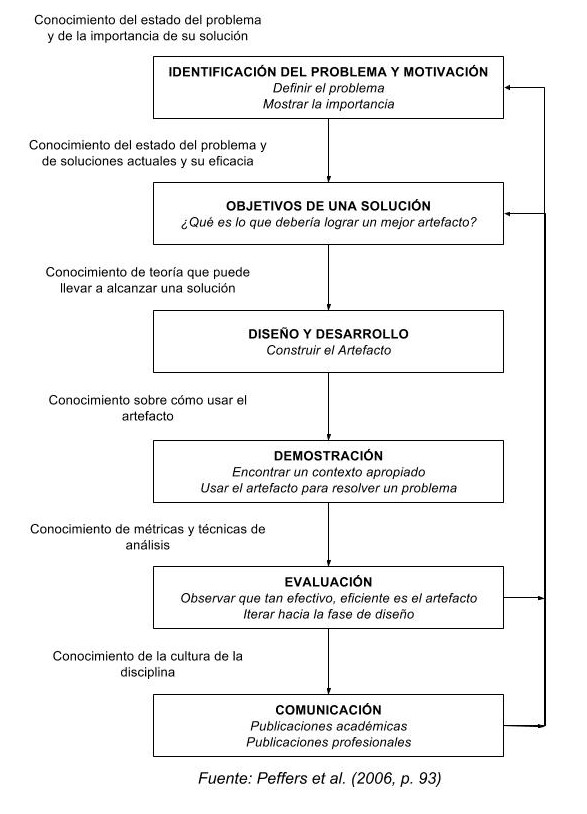
\includegraphics[width=11cm]{graficas/modeloMetodo.jpg}
\end{grafico}
Donde se destaca a \citet[pp. 1127-1128]{dresch2014design}, que apoyados en trabajos previos, entre ellos \citet{vaishnavi2015design} y \citet[p. 56]{peffers2006design}, han señalado que las etapas o pasos principales para realizar investigación basada el paradigma de Ciencia del Diseño, son: la conciencia del problema, sugerencia, desarrollo, evaluación, conclusión, y comunicación. Las salidas (resultados) y la descripción sucinta de dichos pasos se indican en el \refcuadro{tablaModeloCienciaD}, este procedimiento de investigación será utilizado en esta investigación.
\begin{cuadro}[titulo= Etapas principales para realizar investigación en ciencia de diseño, etiqueta = tablaModeloCienciaD]{|p{2cm}|p{4cm}|p{7cm}|}
\hline
 \textbf{Pasos del Proceso} & \textbf{Salidas} & \textbf{Descripción}\\
\hline
Conciencia del problema &
Propuesta 
(incluye formalización del problema, sus límites, y las soluciones que se consideran satisfactorias para el
problema)  &
Se identifica el problema de interés; el investigador debe tratar de comprender el problema para localizar todos sus aspectos y posibles interrelaciones con el contexto en el que está inserto.  \\
\hline
Sugerencia &
Diseño tentativo  &
Se produce un conjunto de posibles artefactos, y se selecciona uno de ellos.  \\
\hline
Desarrollo &
\textbf{Artefacto}  &
Se produce el artefacto, en su estado funcional.  \\
\hline
Evaluación & 
Medidas de desempeño & 
Busca determinar la forma precisa cómo se comporta el artefacto, verificando su habilidad para alcanzar el objetivo deseado. \\
\hline

Conclusiones &
 Resultados &
 Se sintetizan las etapas previas, detallando su proceso de conducción y justificando las elecciones realizadas por el investigador. \\
\hline
Comunicación &
Publicaciones y presentaciones académicas o profesionales (Informes, artículos, memorias, etc.) &
Presentar los resultados de la investigación a las audiencias apropiadas (comunidad académica y organizacional).  \\
\hline
\end{cuadro}
\\
\fuentecuadro{3}{\cite[]{dresch2014design}}\\
Para comprender el tipo de artefactos, \cite[]{lacerda2013design} indican que son objetos artificiales (es decir, creados por humanos), que pueden ser caracterizados en términos de objetivos, funciones y adaptaciones. Además, expresan que los artefactos pueden ser tipificados como: Constructos, Modelos, Métodos e Instanciaciones. Estos autores presentan descripciones de estos tipos de artefactos, como se reseña en el  \refcuadro{tablaArtefacto}.
\begin{cuadro}[titulo= Tipos de artefactos en ciencia de diseño, etiqueta = tablaArtefacto]{|p{4cm}|p{10cm}|}
\hline
 \textbf{Tipos de artefacto} & \textbf{Descripción} \\
\hline
Constructos & 
Constructos o conceptos forman parte del vocabulario de un dominio. Ellos constituyen una conceptualización utilizada para describir los problemas dentro del dominio y especificar las soluciones respectivas. \\
\hline
Modelos & 
Un modelo es un conjunto de proposiciones o declaraciones que expresan las relaciones entre los constructos. En actividades de diseño, los modelos representan situaciones como problema y solución. Puede ser visto como una descripción, o sea, como una representación de las cosas como son. Las ciencias naturales muchas veces usan el término ``modelo'' como sinónimo de ``teoría'', o ``modelos'' como teorías todavía incipientes. \\
\hline
\textbf{Métodos} & 
\textbf{Un método es un conjunto de pasos (un algoritmo u orientación) usado para ejecutar una tarea}. Los métodos se basan en un conjunto de constructos subyacentes (lenguaje) y una representación (modelo) en un espacio de solución. Los métodos pueden estar ligados a los modelos en el sentido de que los pasos pueden utilizar partes del modelo como una entrada que lo compone. \\
\hline
 Instanciaciones &
 Una instanciación es la concretización de un artefacto en su ambiente. Las instanciaciones operacionalizan constructos, modelos y métodos. Sin embargo, una instanciación puede realmente preceder la articulación completa de sus constructos, modelos y métodos subyacentes. Las instanciaciones demuestran la viabilidad y la eficacia de los modelos y métodos que ellas contienen.  \\
\hline
\end{cuadro}
\\
\fuentecuadro{3}{\cite[]{lacerda2013design}}\\

Por lo anteriormente mencionado, el tipo de artefacto a emplear es un método puesto del que se desarrollará un algoritmo conformado por un modelo para sistemas de información de criterios múltiples, utilizado en el área de aplicaciones móviles.

\seccion{Instrumentos de recolección de datos}
Para la recolección de datos, se empleará la técnica de revisión documental, la misma está orientada al tipo de investigación proyectiva. La revisión documental es un proceso que abarca la ubicación, recopilación, selección, revisión, análisis, extracción y registro de información contenida en documentos. Las técnicas de revisión documental pueden ser utilizadas como una vía para la recolección de datos durante una investigación de diseño documental o de fuente mixta, ya sea porque las unidades de estudio son documentos, o porque la información requerida para dar respuesta a la pregunta de investigación ya fue recolectada por otras personas y se encuentra consignada en archivos, registros o cualquier otro tipo de documento \cite[p. 851]{hurtado2012metodologia}. Dentro de las técnicas de revisión documental se utilizarán instrumentos tales como matrices de registro, fichas de observación y matrices de análisis \cite[pp. 855-859]{hurtado2012metodologia}.

\seccion{Instrumentos para el análisis y procesamiento de datos/información}

Para la presente investigación se aplicarán las bitácoras de análisis, técnica descrita por \citet[p.633]{hernandez2010metodologia}  como un instrumento invaluable para la validez y confiabilidad del análisis en información cualitativa. Para la comprobación del algoritmo se utilizará la técnica de simulación por computadora, con un software apropiado para producir las matrices de registros requeridas en esta investigación.\\
\\
Según \citet{hurtado2012metodologia}, la simulación es el proceso de diseñar y desarrollar un modelo computarizado de un sistema o proceso, para realizar experiencias que ayuden a entender el comportamiento del sistema, o evaluar varias estrategias con las cuales se puede operar el mismo. En consecuencia, para llevar a cabo la simulación por computadora, el investigador debe haber construido previamente un modelo explicativo del proceso o la situación a simular, y haberlo expresado en términos matemáticos. Para la creación de modelos, se utilizarán gráficas y fórmulas matemáticas, las técnicas de procesamiento y análisis de información. En el análisis se definirán las técnicas lógicas (inducción, deducción, análisis, síntesis), o estadísticas (descriptivas o inferenciales).

\seccion{Procedimiento de la Investigación}

En el siguiente procedimiento se describen las etapas o fases que se cumplirán para el desarrollo de cada objetivo específico, identificando en cada una de ellas las actividades involucradas y las técnicas a aplicar \cite[p. 11]{UNEXPOmanual2004}.
\begin{enumeracion}
\item[1. ]Para determinar los criterios que deben ser utilizados para la selección de proyectos de aplicaciones  móviles, se efectuarán las siguientes actividades:
\begin{enumeracion}
	\item[a) ] Realizar revisión documental sobre características de sistemas y tecnologías relacionados con la selección de proyectos para aplicaciones móviles.
	\item[b) ] Determinar los criterios representativos para la clasificación de proyectos mediate el uso de matriz de análisis. 
	\item[c) ] Describir los criterios que debe incluir el algoritmo a desarrollar.
\end{enumeracion}
\item[2. ] Para establecer las tareas que han de realizarse para la selección de proyectos de aplicaciones móviles utilizando criterios imprecisos, se hará lo siguiente:
\begin{enumeracion}
	\item[a) ]  Realizar revisión documental sobre métodos, sistemas y tecnologías 	referidos a la selección de proyectos de software en el desarrollo de nuevas aplicaciones móviles para identificar las tareas a incluir en la metodología a utilizar en el algoritmo propuesto.
	\item[b) ]  Describir las tareas que debe incluir el algoritmo a desarrollar.

\end{enumeracion}
\item[3. ]Para conformar el algoritmo que permita realizar las tareas definidas anteriormente, se efectuarán las siguientes actividades:
\begin{enumeracion}
	\item[a) ] Analizar sistemáticamente las tareas para definir los métodos apropiados para conformar el algoritmo propuesto. 
	\item[b) ] Conectar los métodos de manera que conformen un sistema coherente y ordenado. 
	\item[c) ] Especificar el método apropiado para llevar a cabo las tareas requeridas.
	\item[d) ] Validar el método especificado.
\end{enumeracion}

\item[4. ] Para evaluar el algoritmo propuesto, se realizarán las actividades señaladas a continuación:	
\begin{enumeracion}
	\item[a) ] Implementar 	un prototipo de sistema basado en el algoritmo propuesto. 
	\item[b) ]Elegir 	un caso representativo de selección de alternativas.
	\item[c) ]Realizar experimentos con el caso representativo, utilizando el prototipo de sistema basado en el algoritmo propuesta.
	\item[d) ]Analizar los resultados obtenidos del experimento realizado.
\end{enumeracion}
\item[5. ] Adicionalmente a las actividades anteriores, las cuales se efectúan para alcanzar los objetivos específicos, se llevará a cabo lo siguiente:
\begin{enumeracion}
	\item[a) ] Elaborar el Trabajo de Grado. 
	\item[b) ] Defender el Trabajo de Grado.
	\item[c) ] Elaborar la versión Final del Trabajo de Grado para optar al grado de Magíster Scientiarum
\end{enumeracion}
\end{enumeracion}
\\
A continuacion se ilustra el procedimiento de la presente investigación en el marco de la investigación de la ciencia del diseño, indicando las actividades por fases, así como las técnicas y procedimientos a utilizar, y los resultados parciales esperados.
\newpage
\subseccion{ Fase I. Determinar los criterios a incluir en el algoritmo}
\begin{cuadro}[sinleyenda, sinindice]{|p{6cm}|p{2.5cm}|p{4cm}|}
\hline
\textbf{Actividad  y/o Técnica} & \textbf{Instrumento} & \textbf{Resultado parcial esperado}\\
\hline
a) Realizar revisión documental sobre características de sistemas y tecnologías relacionados con la selección de proyectos para aplicaciones móviles.
 &  Revisión documental & Conocimiento sobre los criterios a incluir en el algoritmo a proponer.
  \\
  \hline
b)  Determinar los criterios representativos para la clasificación de proyectos. 
  & Lista de cotejo / Fichas de observación / Matrices de análisis 
  & Identificación de criterios a ser utilizados en el algoritmo. \\
  \hline
c) Describir los criterios que debe incluir el algoritmo a desarrollar. 
 &  Matrices de análisis
 & Información sobre características de los criterios a incluir \\
\hline
\end{cuadro}
\subseccion{ Fase II. Establecer las tareas a incluir en el algoritmo}

\begin{cuadro}[sinleyenda, sinindice]{|p{6cm}|p{2.5cm}|p{4cm}|}
\hline
\textbf{Actividad  y/o Técnica} & \textbf{Instrumento} & \textbf{Resultado parcial esperado}\\
\hline
d) Realizar revisión documental sobre métodos y sistemas relacionados con metodología a diseñar.
 & Revisión documental/ matrices de análisis de contenido
 & Conocimiento sobre las tareas a incluir en metodología a diseñar  \\
\hline
e) Describir las tareas a incluir 
 & Revisión documental/ matrices de análisis
 & Información sobre características de las tareas a incluir  \\
\hline
\end{cuadro}
\newpage
\subseccion{ Fase III. Conformación del algoritmo que permita realizar las tareas}
\begin{cuadro}[sinleyenda, sinindice]{|p{6cm}|p{2.5cm}|p{4cm}|}
\hline
\textbf{Actividad  y/o Técnica} & \textbf{Instrumento} & \textbf{Resultado parcial esperado}\\
\hline
f) Analizar sistemáticamente las tareas para definir los métodos apropiados.
 &  Matrices de análisis
 &  Definición de métodos apropiados para realizar las tareas y criterios asociados \\
\hline
g) Conectar los métodos de manera que conformen un sistema coherente y ordenado.
 & Matrices de análisis
 & Esquema representativo de la estructura del algoritmo.  \\
\hline
h) Especificar el método apropiado para llevar a cabo las tareas requeridas 
 & Análisis, síntesis 
 & Especificado el método apropiado del algoritmo.\\
\hline
i) Validar el método especificado &  Simulación por computadora &  Validación del Método especificado \\
\hline
\end{cuadro}
\subseccion{ Fase IV. Prueba del algoritmo propuesto}

\begin{cuadro}[sinleyenda, sinindice]{|p{5cm}|p{2.5cm}|p{5cm}|}
\hline
\textbf{Actividad  y/o Técnica} & \textbf{Instrumento} & \textbf{Resultado parcial esperado}\\
\hline
j) Implementar 	un prototipo de sistema basado en el algoritmo propuesto. 
 & Análisis, síntesis
 & Prototipo del algoritmo diseñado \\
\hline
k) Elegir 	un conjunto representativo de casos  e selección de alternativas. & Análisis, síntesis
 & Conjunto representativo de casos de selección de proyectos para la selección de proyectos de aplicaciones móviles. \\
\hline
l) Realizar experimentos con un caso de prueba, utilizando el prototipo de sistema basado en el algoritmo diseñado     
 & Simulación por computadora/ computadora, matrices de registro 
 & Indicador de eficacia de la propuesta \\
 \hline

\end{cuadro}
\begin{cuadro}[sinleyenda, sinindice]{|p{5cm}|p{2.5cm}|p{5cm}|}
\hline
m) Analizar los resultados obtenidos de los experimentos realizados
 & Análisis, síntesis & Información útil para mejorar el algoritmo\\
 \hline
\end{cuadro}

\subseccion{ Fase V. Comunicación de los resultados obtenidos}




\begin{cuadro}[sinleyenda, sinindice]{|p{6cm}|p{2.5cm}|p{4cm}|}
\hline
\textbf{Actividad  y/o Técnica} & \textbf{Instrumento} & \textbf{Resultado parcial esperado}\\
\hline
n) Elaborar la Tesis de Maestría & Redacción de informes científicos &  Tesis de Maestría elaborada \\
\hline
o) Defender la Tesis de Maestría & Argumentación científica & Tesis defendida \\
\hline
p) Elaborar la versión final de la Tesis de Maestría & Redacción de informes científicos & Versión final elaborada  \\
\hline
\end{cuadro}